\chapter{Kernel Density Estimates for Generating Mock Type Ia Supernova Observations with SALT2 and SNEMO}
\label{chap:kde}

\section{Overview}
As discussed in Chapter \ref{chap:intro}, the most common method currently for calibrating supernova brightnesses for cosmology uses the SALT2 spectral model of \cite{guy_salt2_2007} along with an assumed linear relationship between the model parameters and absolute magnitude at maximum brightness. The SALT2 model assumes that the flux $f_{mod}$ at wavelength $\lambda$ and phase $p$ is given by
\begin{equation}
    f_{mod}(\lambda, p) = x_0 \left[M_0(\lambda, p) + x_1\;M_1(\lambda, p)\right] \times \exp\left[c\;CL(\lambda)\right]
    \label{eqn:salt_flux_model}
\end{equation}
where $x_0$, $x_1$, and $c$ are parameters approximately describing the overall scale, light curve decay rate, and color of each supernova respectively, $M_0(\lambda, p)$ and $M_1(\lambda, p)$ are functions of wavelength and phase describing the average spectral sequence of SNe~Ia and typical variance SN spectral sequences, and $CL$ is a function of wavelength, representing the effects of both intrinsic and extrinsic color variation on observed flux. In a typical analysis, each observed light curve is fit with this model, giving $x_0$, $x_1$, and $c$ values for each supernova. The distance modulus to each supernova is then modeled linearly \citep{tripp_two-parameter_1998, tripp_determination_1999} by
\begin{equation}
    \mu = m_B^* + \alpha x_1 -\beta c - M
\end{equation}
where $m_B^*$ is the apparent magnitude in the Bessell B-band at maximum brightness of a supernova with the observed $x_0$, $x_1$, and $c$ (as predicted by the SALT2 model), and $\alpha$, $\beta$, and $M$ are global standardization parameters obtained from a simultaneous fit of $\mu$ and the distance modulus as a function of cosmological parameters.

After parametrizing the light curves with the SALT2 model and accounting for empirical relations between these parameters and luminosity, there still is scatter of approximately 0.14 mag remaining in the standardized magnitudes. Some portion of this scatter may be intrinsic, but several studies have shown that at least some of the scatter stems from flawed assumptions of the model, as we now discuss.

Firstly, the light curve parametrizations themselves do not capture all of the diverse ways that observable supernova properties correlate with luminosity. The supernova twins analysis of \cite{fakhouri_improving_2015} points to this particular problem with the standard SALT2 analysis pipeline by showing that a direct comparison of maximum brightness spectra, without any parametrization of the broadband light curves, results in a smaller scatter in standardized brightnesses. The existence of spectral subclasses of Type Ia supernovae (e.g. \cite{branch_comparative_2006}) also suggest that there is more information contained within the spectra of SNe~Ia than the SALT2 model is capturing. The SuperNova Empirical Models (SNEMO, \cite{saunders_snemo_2018}; described in more detail in Section~\ref{sec:snemo}) were introduced in part to mitigate the effects of using such incomplete models of supernova variation by including additional time-series flux components.

Even with a perfectly descriptive supernova flux model, a straight-forward linear relation may be unable to capture all of the details of the relationship between model parameters and luminosity, resulting in additional unexplained dispersion in standardized magnitudes. For example, \cite{rubin_unity_2015} found a preference for a broken-linear relationship between light curve color and luminosity. \cite{rose_initial_2020} showed that a non-linear Gaussian process may better encapsulate the relationship between SN color and absolute luminosity. This issue has been significantly less well-studied than the inflexibility of the flux models, but further studies would require improved simulations to understand the relative fraction of uncertainty stemming from the inflexibility of the flux parametrization model as opposed to the inflexibility of the standardization model.

Both of these issues are further complicated by selection effects and observational error. Without accounting for these uncertainties and propagating them through the analysis, the resulting cosmological parameter measurements are potentially biased. In order to have accurate simulations to quantify and correct for these biases, we must have a data-informed model of the underlying parameter populations. Indeed, \cite{scolnic_measuring_2016} show that using incorrect estimates of the underlying stretch and color distributions of the SALT2 parameters results in a small bias in the dark energy equation-of-state parameter, $w$. Simulations are an important tool for quantitatively disentangling the intrinsic scatter from the flux parametrization error and supernova standardization error; creating tools for these more descriptive simulations is the main motivating factor of this work.

In this analysis, we present a tool for flexibly estimating the underlying population distributions of the model parameters for the SALT2 and SNEMO models in order to build accurate simulations that can address some of these issues. We present an overview of the SNEMO model in Section~\ref{sec:snemo} and discuss the collection of spectro-photometric time-series data that we use throughout the analysis in Section~\ref{sec:data}. In Section~\ref{sec:kde}, we present the general framework for estimating latent joint probability distributions and the methods for quantitatively comparing these estimates to the simpler distribution estimation models like a multivariate Gaussian. We apply this methodology to our data and explain how to move from these parameter distribution estimates to mock observations in Section~\ref{sec:making_mocks}. Finally, we compare the distributions of maximum-brightness spectral feature measurements in Section~\ref{sec:spec_diversity}, and conclude with some proposed further analyses in Section~\ref{sec:conclusions}.

\section{SNEMO}
\label{sec:snemo}
Again as we discussed in Chapter \ref{chap:intro}, the SuperNova Empirical MOdels (SNEMO) are a family of linear models that were built to capture more of the spectral variation than is captured by fewer-parameter models like SALT2. The mathematical form of the SNEMO flux model is very similar to that of SALT2, but with a larger number of parameters. The flux at wavelength $\lambda$ and phase $p$ is modeled by
\begin{equation}
    f_\text{mod}(\lambda, p) = c_0 \left[e_0(\lambda, p) + \displaystyle\sum_{i=1}^k c_i\;e_i(\lambda, p)\right] \times 10^{-0.4 A_s CL(\lambda)}
\label{eqn:snemo_flux_model}
\end{equation}
where $e_0(\lambda, p)$ is the average spectral sequence, and each of the $e_i(\lambda, p)$ represent orthogonal aspects of spectral variation. $CL(\lambda)$ is the \cite{fitzpatrick_correcting_1999} extinction relation and is fixed across all time scales to represent extinction from dust. The model parameters are then the overall scaling $c_0$, the variational parameters $c_i$ and the dust-reddening parameter $A_s$. These $k+1$ parameters represent the full spectral time-series data in the model space, similar to how the parameters $\{x_0, x_1, c\}$ represent the time-series of supernova spectra in the SALT2 model.

\cite{saunders_snemo_2018} presents three different variations of the model, each with different numbers of parameters and intended for different uses. SNEMO2 has a single spectral variation vector ($k=1$) in addition to the overall scale and color parameters, and serves as a point of comparison to SALT2. SNEMO7 has six spectral variation vectors ($k=6$) and is presented as a model for supernova standardization, as it minimizes the unexplained dispersion in standardized magnitudes of supernovae after using the coefficients of this model to linearly standardize the luminosity. Finally, SNEMO15 ($k=14$) is presented as a model to explain as much of the spectral variability as possible, as measured by the total $\chi^2$ difference between the model and the observed fluxes at all of the modeled wavelengths and phases. Throughout this work, we make use of and compare each of these three models along with the SALT2 model.

\section{Data}
\label{sec:data}
In order to generate new spectral time-series data from this model, we first need measurements of the spectral model parameters from a representative data set. The representative data set we are using throughout this analysis is the spectral time-series data from the Nearby Supernova Factory \citep[SNfactory;][]{aldering_overview_2002}. SNfactory has collected spectrophotometry from over 400 SNe~Ia. Of these, 228 are considered high quality enough for light curve fitting, and have light curve parameters within the typical ranges used in cosmology analyses.\footnote{This analysis is based on the \texttt{CASCADE} production of the SNfactory pipeline.} With each spectral model (SALT2 and each SNEMO model), we obtain a vector of model parameters for each supernova by minimizing
\begin{equation}
    \chi^2 = \displaystyle\sum_{\lambda, p} f_\text{obs}(\lambda, p) - f_\text{mod}(\lambda, p\;|\; \Theta)
\end{equation}
with respect to the model parameters $\Theta$, where $f_{obs}$ is the observed flux (after correcting for Milky Way dust extinction), and $f_{mod}$ is the model flux from Eqn. \ref{eqn:salt_flux_model} for SALT2 or Eqn. \ref{eqn:snemo_flux_model} for the SNEMO models.

The overall scaling parameter ($x_0$ for the SALT2 model and $c_0$ for the SNEMO models) measured for each supernova depends not only on the absolute magnitude of the object, but also on the object's redshift. We would like our generative model to be able capture the range of intrinsic absolute magnitude fluctuations irrespective of the redshift and to include correlations between these fluctuations and the spectral model parameters. To accomplish this, we convert these scaling parameter value to a value representing the absolute magnitude of each object (which we denote by $M_B^*$) by calculating the apparent magnitude in the Bessell B-band at maximum brightness of a supernova with the best-fit $x_1$ and $c$ (or $c_i$ and $A_s$) values and subtracting the distance modulus to an object at the same redshift assuming a fixed, fiducial $\Lambda$CDM cosmology with $H_0=70$ km/s/Mpc and $\Omega_{m}=0.3$. To simplify our plots and our kernel density estimates, we subtract a typical value of this parameter ($\langle M_B^*\rangle \approx -19.1$).

% Table~\ref{tab:snemo_coefs} presents a truncated table with the SALT2, SNEMO2, SNEMO7, and SNEMO15 coefficients for each supernova in the data set, along with their $M_B^*$ values. The full-table is available online.

% \include{data/BLACKSTONE_fits_published_snemo_and_salt}

\section{Kernel Density Estimation}
\label{sec:kde}
With these measurements in hand, we move on to estimating the underlying joint probability distribution of these observations. Kernel density estimation is one such method for making these approximations. Simply put, provides an estimate fo the joint probability distribution by weighting each of the observed data points by some kernel function $k(\bm{x}_{1}, \bm{x}_{2})$ and summing these weights to produce a smooth curve representing the probability density across parameter space \citep{silverman_density_1986, wand_kernel_1995, scott_multivariate_2014}. Although the resulting estimate of the latent probability distribution is non-parametric, the kernel function used is usually parametrized by a parameter known as the bandwidth. This hyperparameter controls the level of smoothing by controlling the relative weights of data points spread further apart; in the case of a one-dimensional Gaussian kernel, this is the standard deviation of the Gaussian, $\sigma$.

Typically, this parameter is determined through $k$-fold cross-validation. In $k$-fold cross validation, the sample is first split into $k$ groups. One of these groups is held out while the model is trained on the data in the remaining groups, and then evaluated via some scoring metric on the held-out set. This process is repeated for a range of model hyperparameters, and the best values of the hyperparameters are those that maximize the average score on the held out set. In our case, we use the sum of log likelihoods of the test data under the model fit using the training data as our scoring metric.

In Appendix \ref{sec:1d}, we provide a detailed example of using this process to fit a KDE to a one-dimensional probability distribution. Finding the proper bandwidth matrix to fit a KDE in multiple dimensions is slightly more complicated. However, we can reduce the problem of bandwidth selection in many dimensions to the problem of bandwidth selection in one dimension by finding a whitening matrix, which defines a linear transformation of the data so that the covariance matrix of the transformed data is proportional to the identity matrix. Applying this transformation, fitting a KDE with the ideal bandwidth for this transformed data, and inverting the transformation gives us the desired fit. Appendix \ref{sec:2d} contains a detailed two-dimensional example, including a proof of a form of the whitening matrix.

\section{Modeling the Data and Making Mock Observations}
\label{sec:making_mocks}
\subsection{Comparing Parameter Distributions}
We apply the multidimensional KDE fitting process with 5-fold cross validation of the bandwidth to the spectral model parameter measurements found in Section~\ref{sec:data}. Corner plots of the data points and similarly sized samples drawn from the resulting transformed KDE are shown in Figs. \ref{fig:salt2_sample}-\ref{fig:snemo15_sample}.

\begin{figure}
    \centering
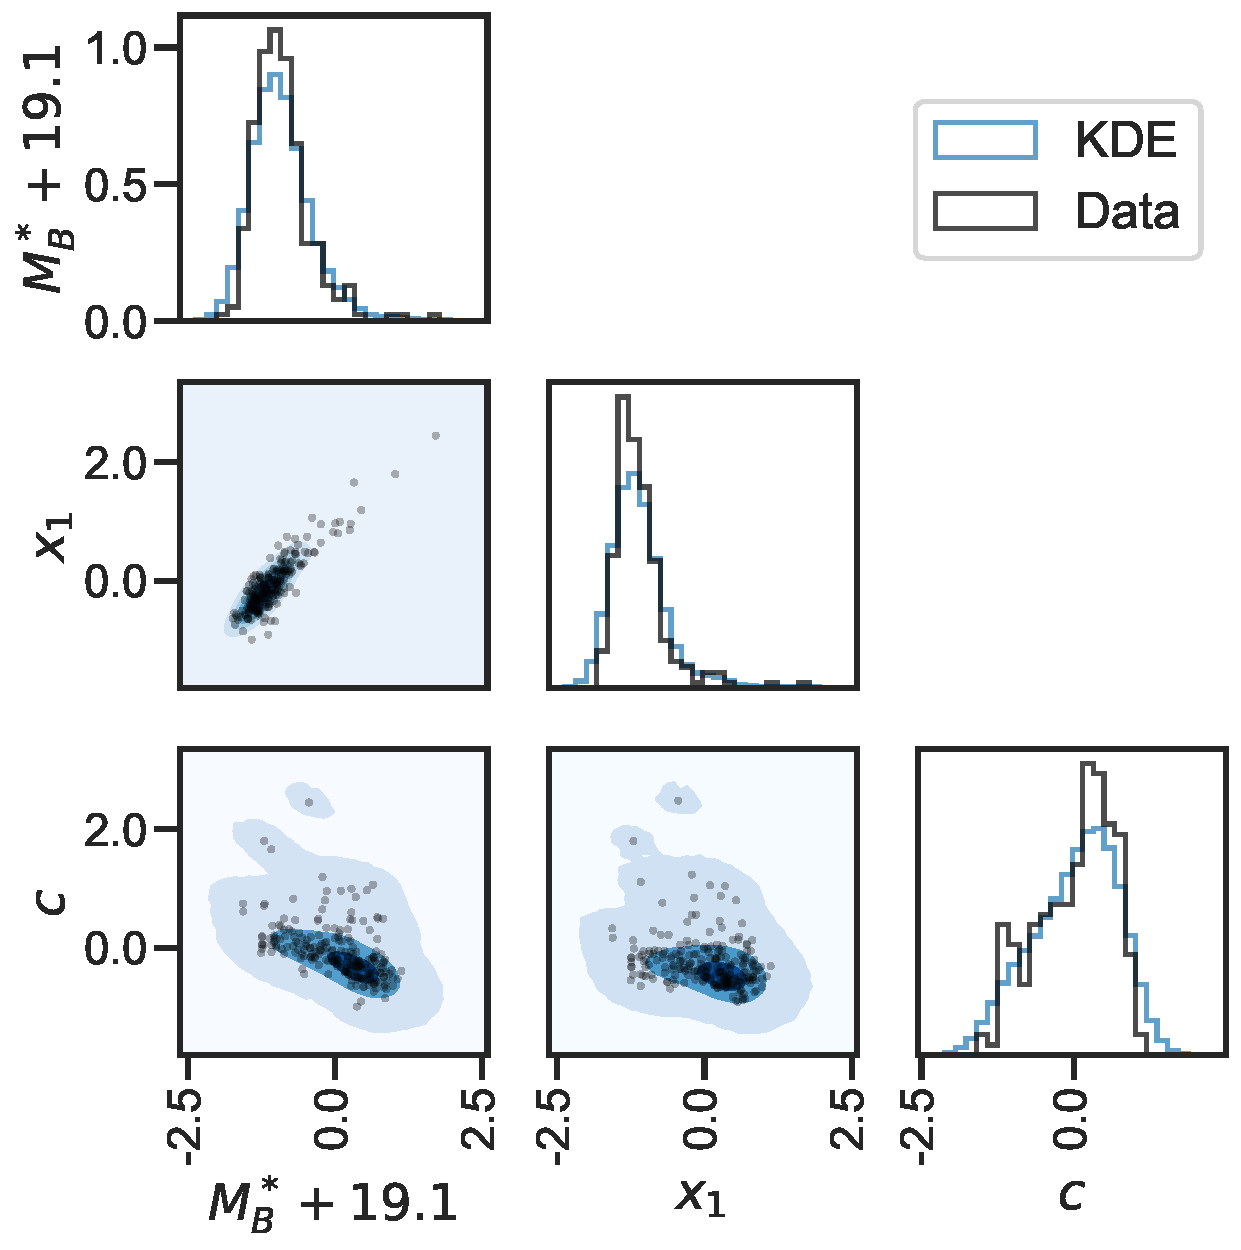
\includegraphics[width=0.9\textwidth]{figures/snemo_kde/salt2_blob_corner.pdf}
    \caption{Corner plot showing the one- and two-dimensional marginal parameter distributions of the SALT2 parameters for the SNfactory data set (black points and histogram lines), as well as the 1-, 2-, and 3-$\sigma$ confidence intervals of the marginalized distribution of samples drawn from the KDE trained on these data.}
    \label{fig:salt2_sample}
\end{figure}

\begin{figure}
    \centering
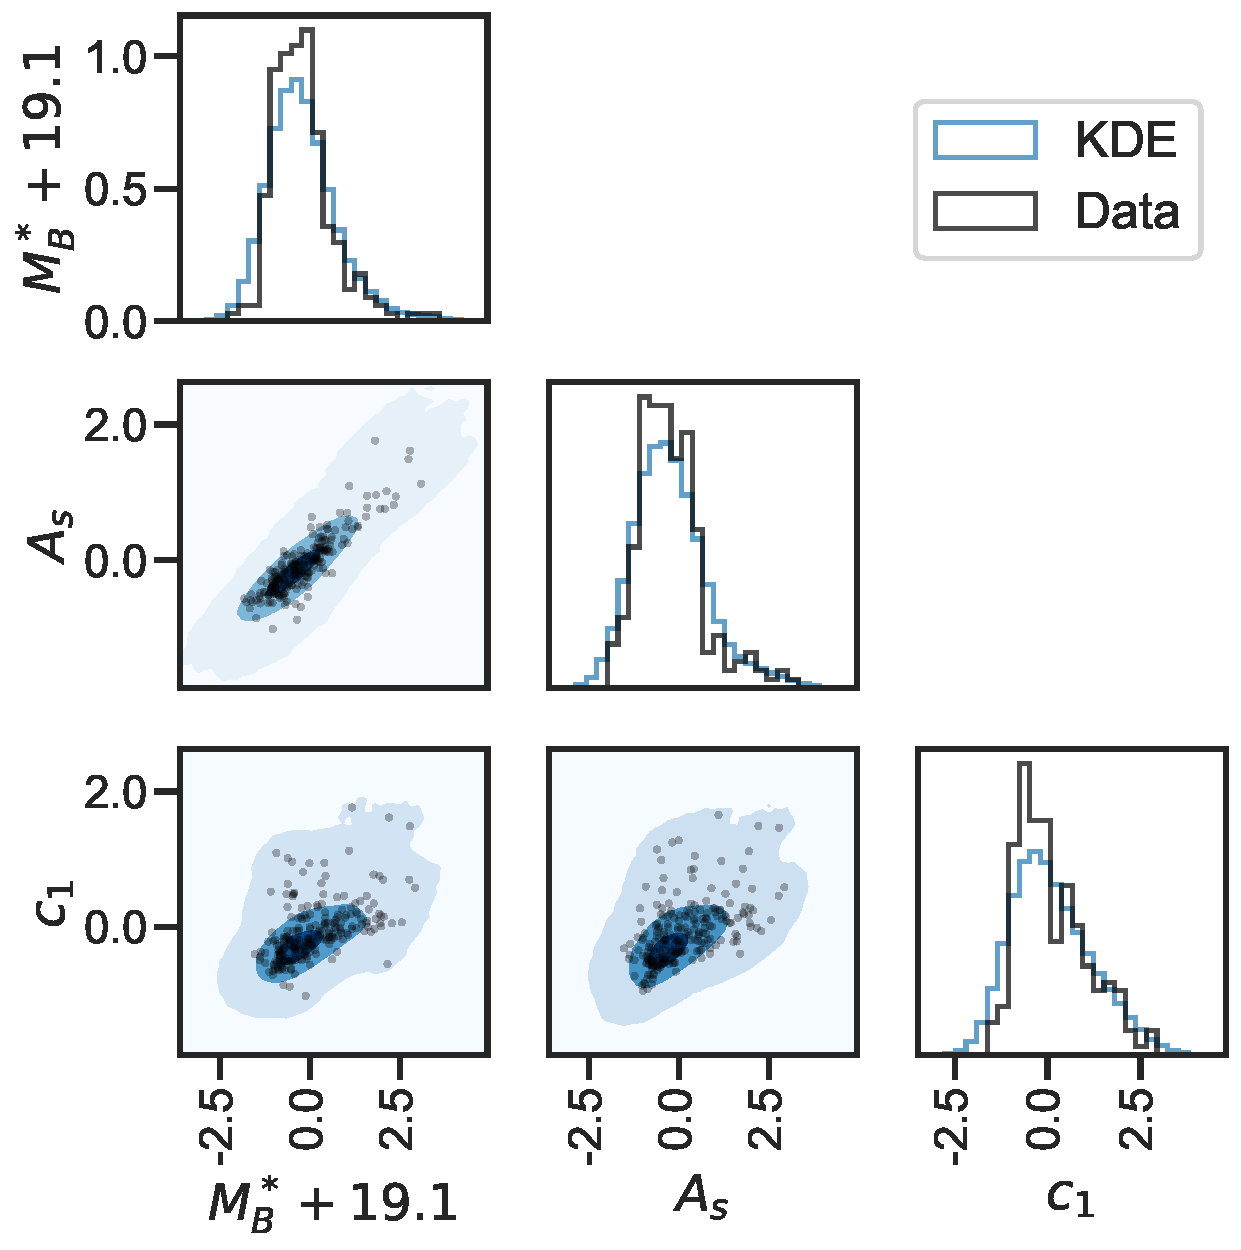
\includegraphics[width=0.9\textwidth]{figures/snemo_kde/snemo2_blob_corner.pdf}
    \caption{Same as Fig.~\ref{fig:salt2_sample}, but for SNEMO2}
    \label{fig:snemo2_sample}
\end{figure}

\begin{figure}
    \centering
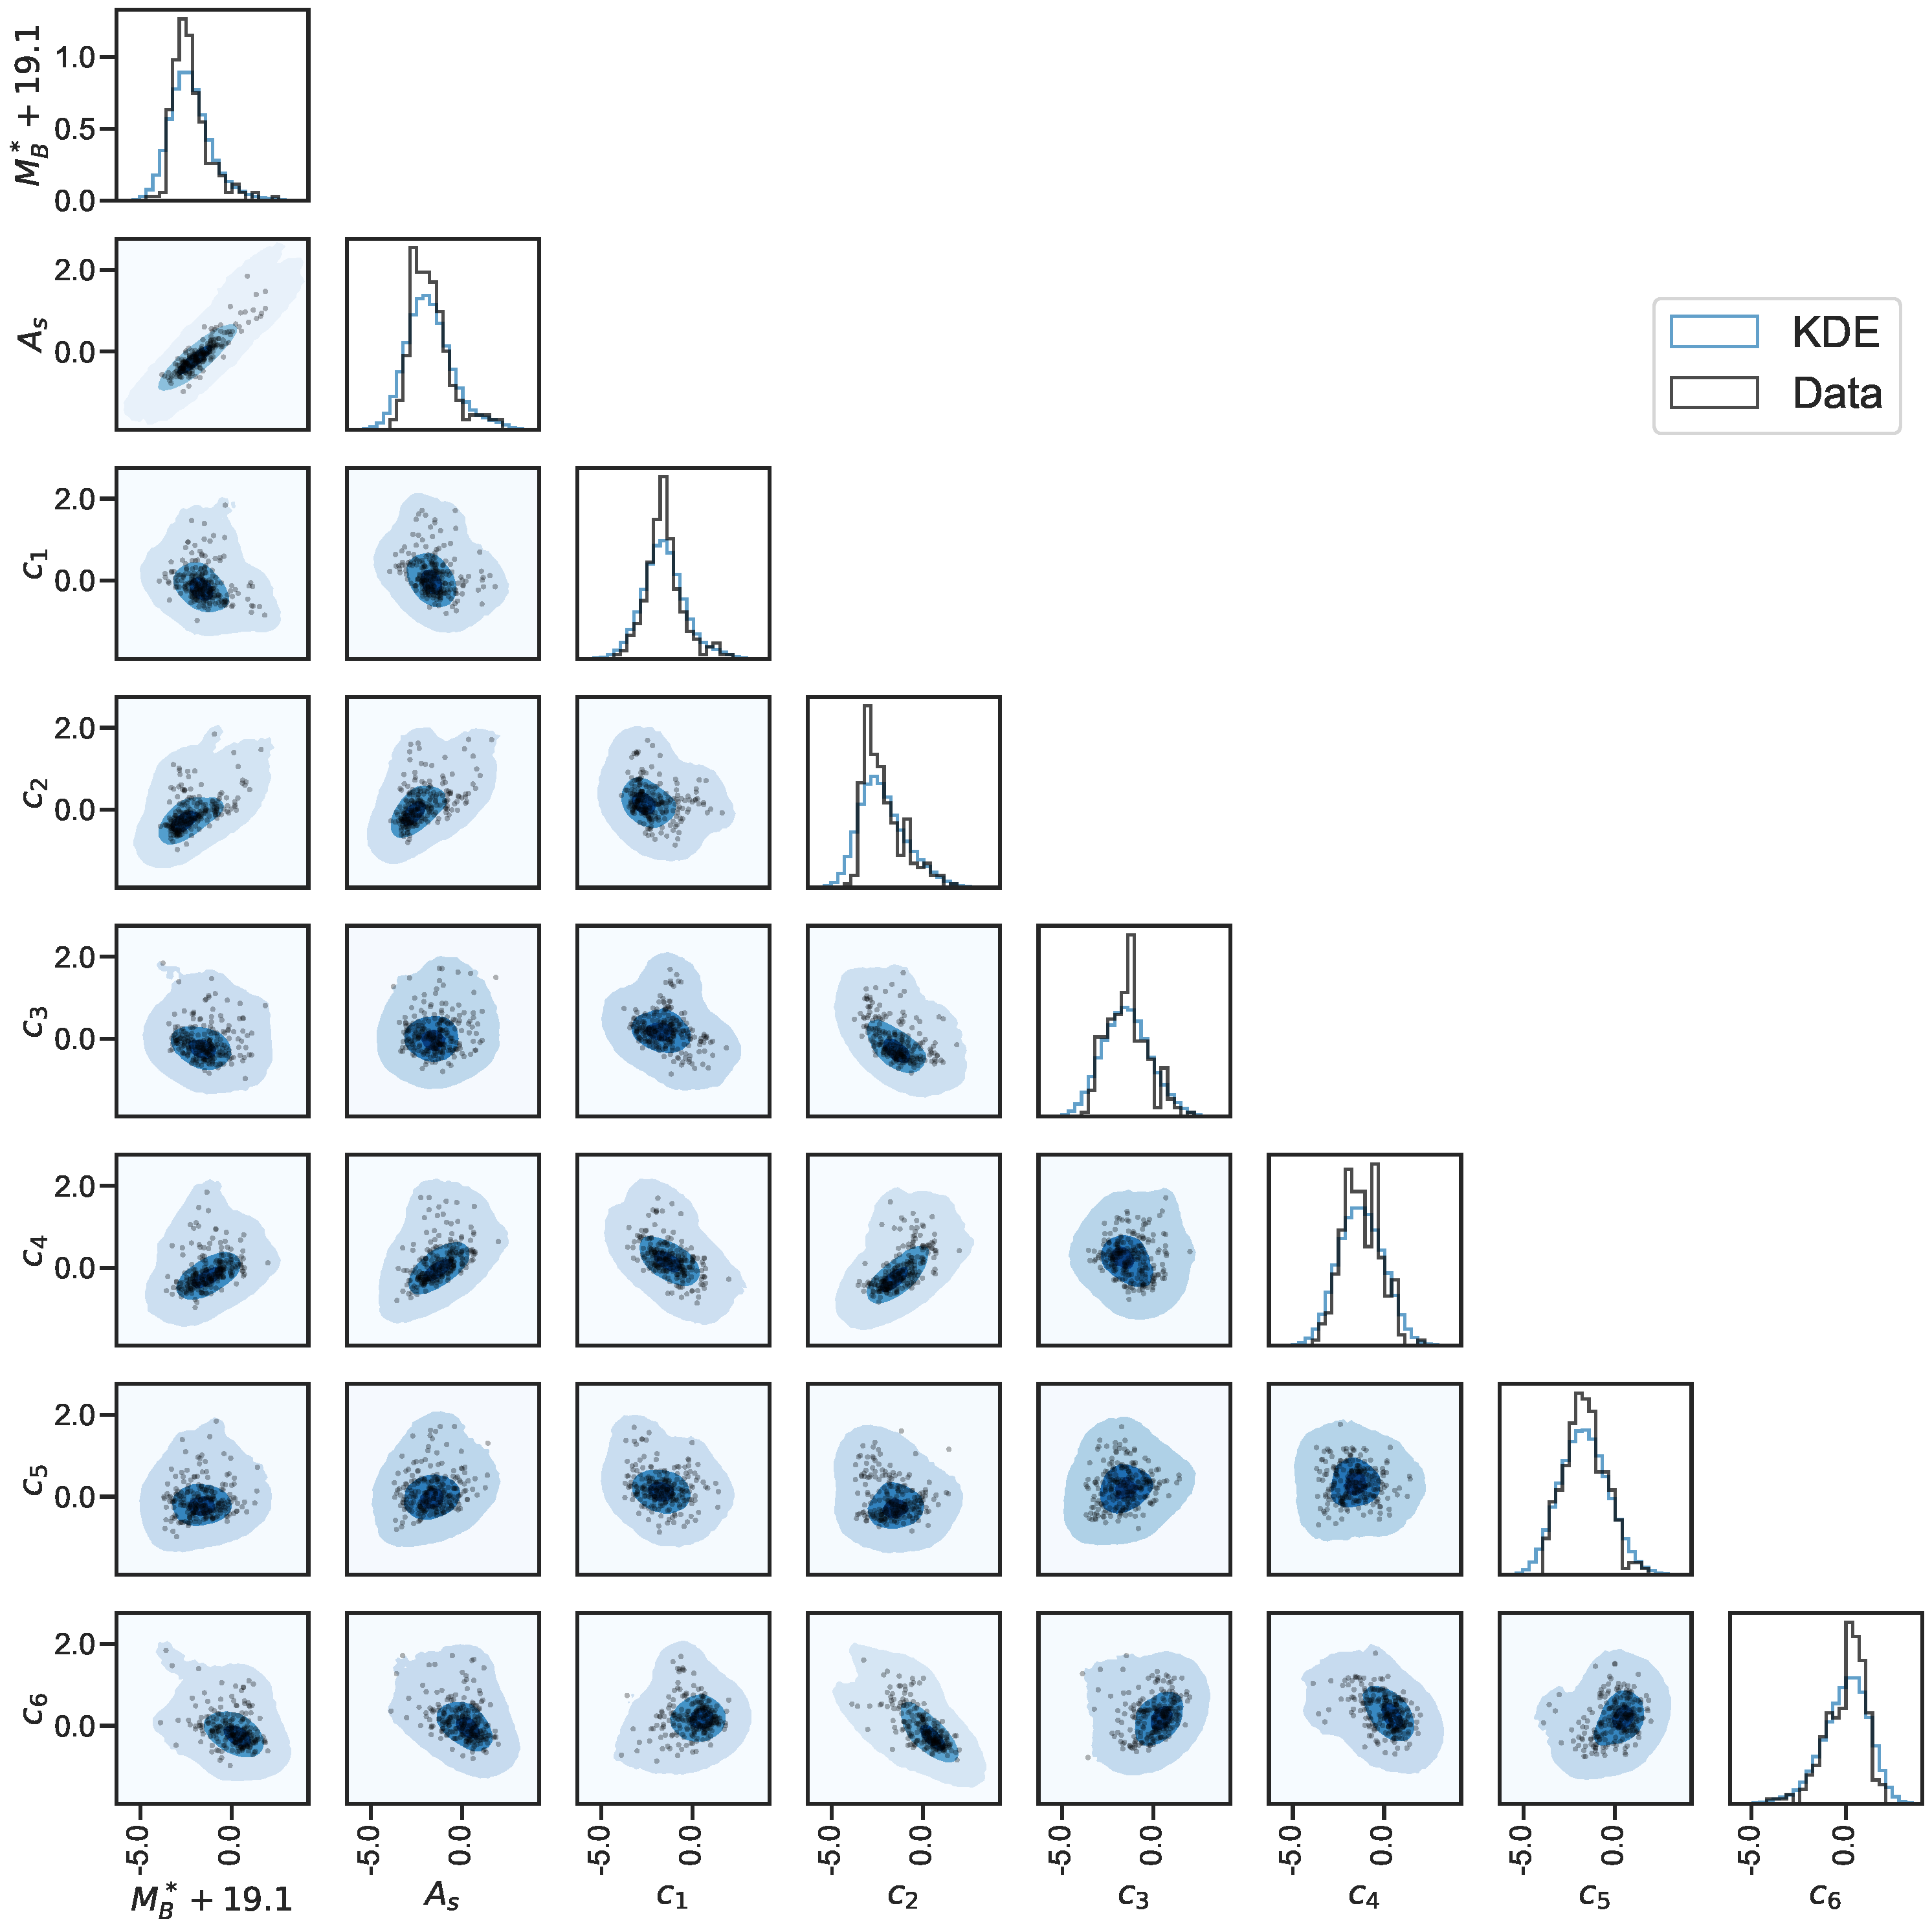
\includegraphics[width=0.9\textwidth]{figures/snemo_kde/snemo7_blob_corner.pdf}
    \caption{Same as Fig.~\ref{fig:salt2_sample}, but for SNEMO7}
    \label{fig:snemo7_sample}
\end{figure}

\begin{figure}
    \centering
\includegraphics[width=0.9\textwidth]{figures/snemo_kde/snemo15_blob_corner.pdf}
    \caption{Same as Fig.~\ref{fig:salt2_sample}, but for SNEMO15}
    \label{fig:snemo15_sample}
\end{figure}

By eye, the marginal probability distributions of of the KDE samples appear to match the data quite well across all models. This is true even of the skewed parameter distributions, like those corresponding to the color terms in the model (SALT2 $c$ and SNEMO $A_s$). The two-dimensional marginalized distributions are also visually close to those of the data, even when the distributions deviate from a Gaussian, as they do for $c_1$ and $c_2$, for example, in SNEMO7. In Section \ref{sec:spec_diversity}, we quantify these qualitative descriptions by comparing the distributions of spectral feature indicators from the data to the distributions obtained from spectra simulated using the KDE model and a multivariate Gaussian model of the spectral model parameters.

% Calculating this distance in many dimensions is possible, but computationally difficult because of memory limitations associated with calculating large dimensional histograms. Therefore, we chose to compare each of the \emph{marginalized} distributions of each spectral model parameter. The Cram\'{e}r distances between the spectral model parameter marginal distributions from the best-fit KDE and from the data, as well as corresponding distances where a simple multivariate Gaussian replaces the KDE, are presented in Fig.~\ref{fig:distances}.

% \begin{figure}
%     \centering
%     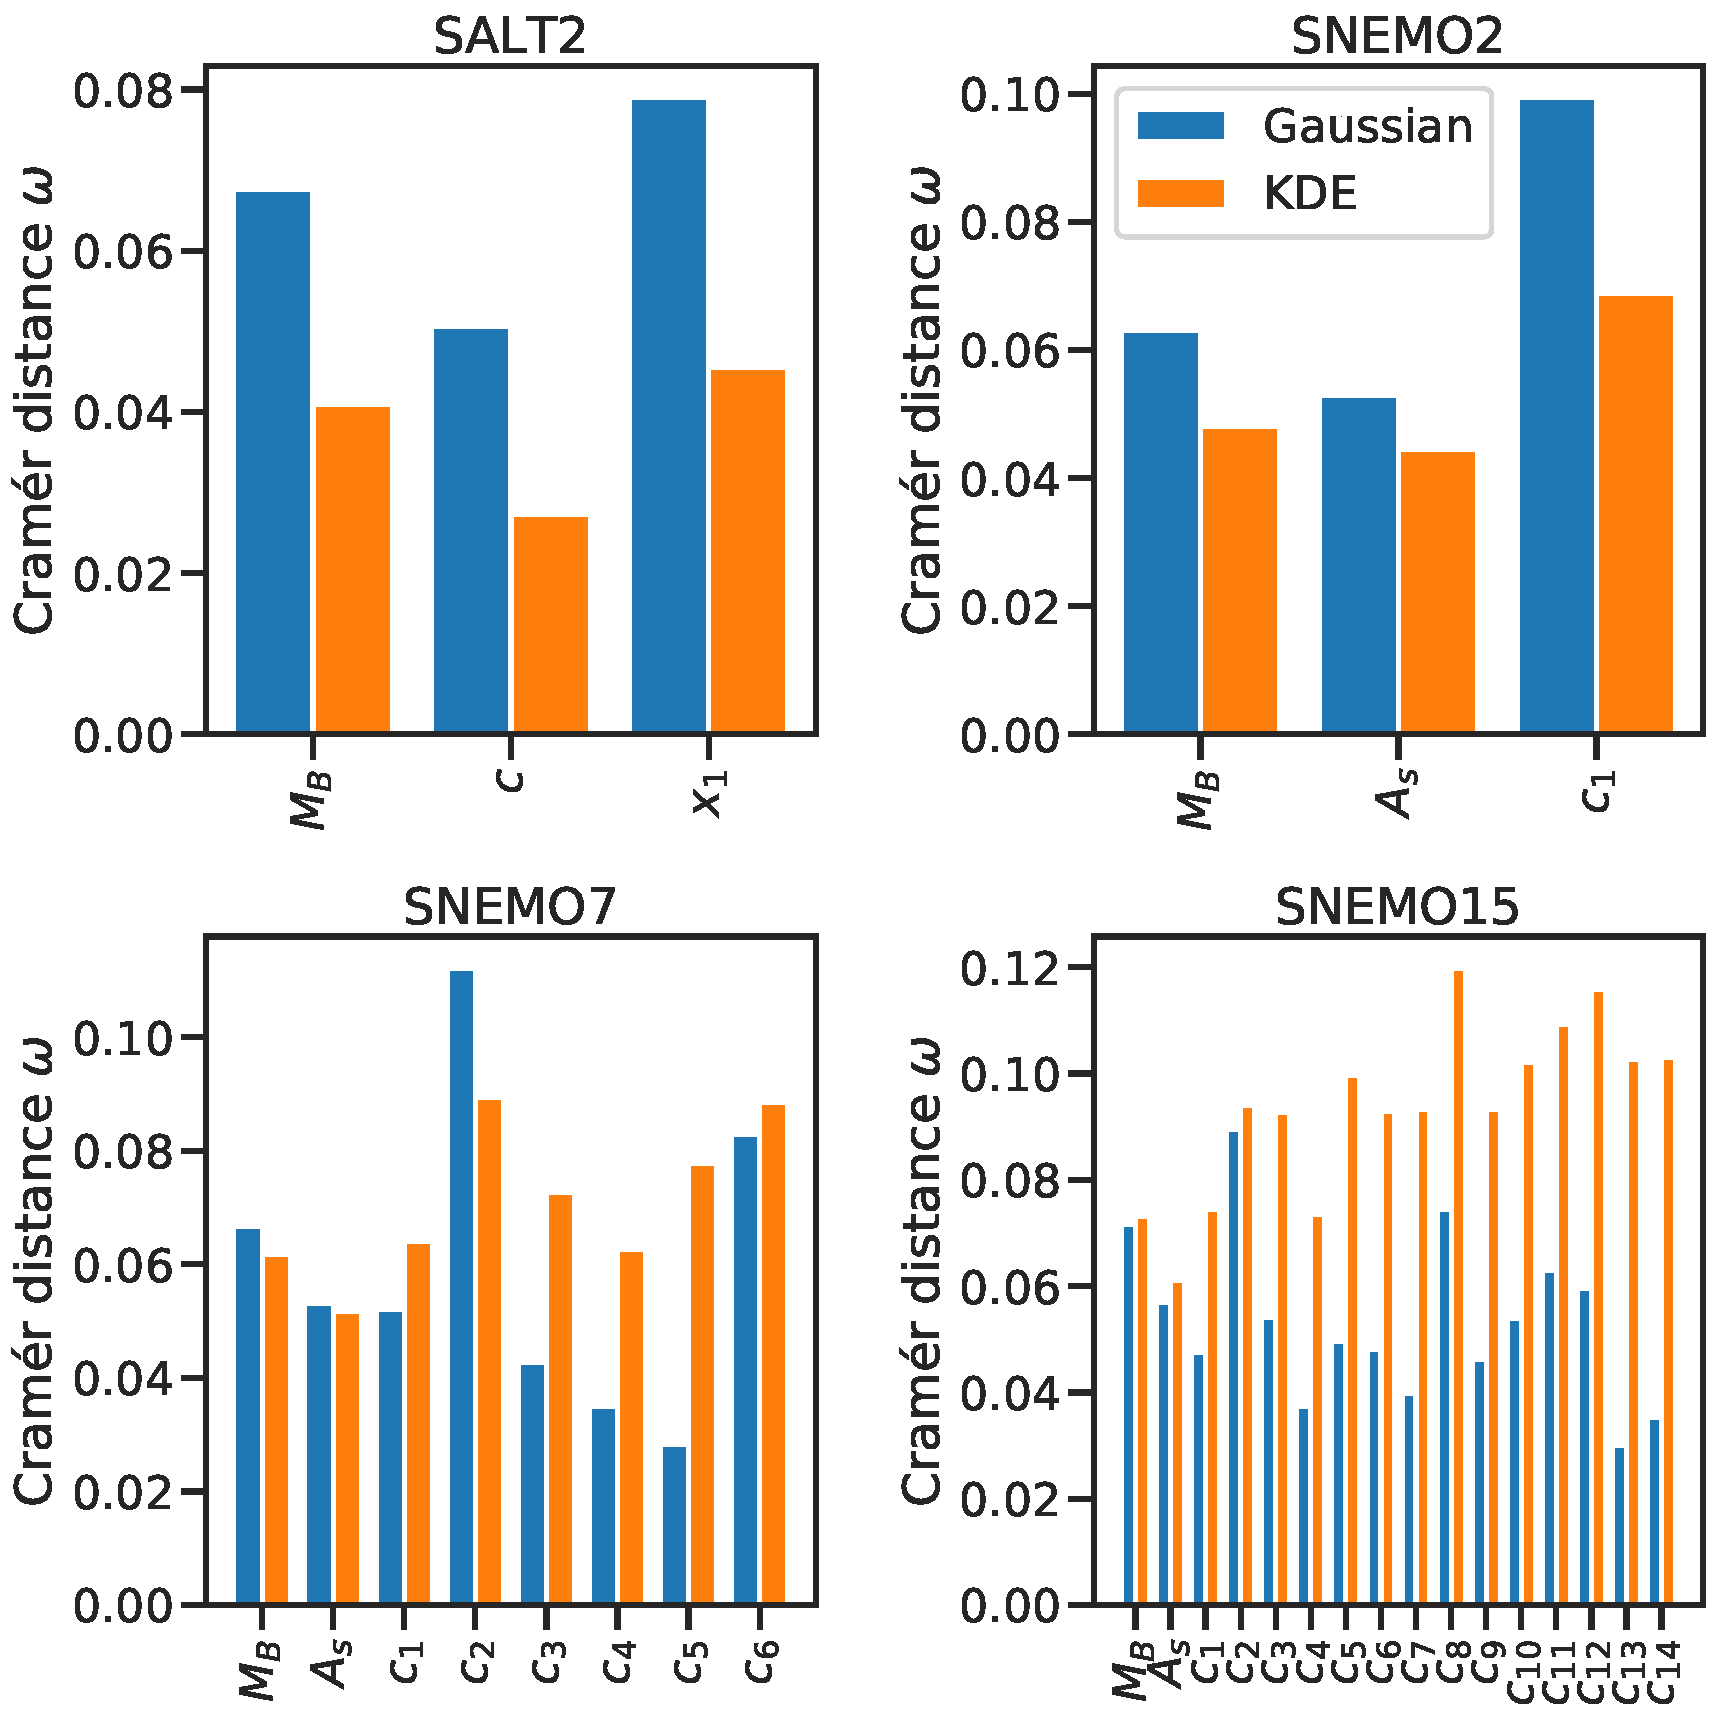
\includegraphics[width=0.9\textwidth]{figures/snemo_kde/cramer_distances_param_space.pdf}
%     \caption{Cram\'{e}r distances between the empirical marginal distributions functions of the data sample and samples from a multivariate Gaussian (blue) and samples from the KDE (orange) for each parameter in each of the spectral models studied.}
%     \label{fig:distances}
% \end{figure}

% In the fewer-parameter models (SNEMO2 and SALT2), the marginal distributions of the parameters found with the KDEs match those from the data much better than those drawn from a simple multivariate Gaussian. For SNEMO7, some of the marginalized parameter distributions, like $c_2$, are better described by the KDE than the Gaussian. Others, however, are better approximated by a Gaussian distribution. For SNEMO15, each of the marginalized parameter distributions are better modeled by Gaussians than they are by the marginalized KDEs. 

% It is important to note that the metric we are using uses only the information from the marginalized probability distributions, and therefore cannot account for skewness and non-Gaussianity in the joint probability distributions. As an example of this effect, we show the observed 2-dimensional joint distribution of SNEMO15 $A_s$ and $c_1$, along with contour plots of the same distribution given by the KDE and a multivariate Gaussian in Fig.~\ref{fig:snemo15_joint_example}. While the Cram\'{e}r distance between the data and the marginalized KDE distributions of these two parameters is larger than the distance between the data and the marginalized Gaussian distribution, we see visually that the KDE seems to better capture the deviations from pure Gaussianity in the joint distributions, as evidenced by the closer agreement of the modes of the distributions and incorporation of larger tails in the distribution. Moreover, we will see in Section~\ref{sec:spec_diversity} that using the KDE to model the spectral model parameter space allows us to capture a more realistic range of spectral feature measurements. The distances presented are meant to serve as a rough heuristic for the agreement between the distributions found by this technique and the data. A more detailed look, perhaps exploring the Cram\'{e}r distances in the two-dimensional distributions, is left to future work.

% \begin{figure}
%     \centering
%     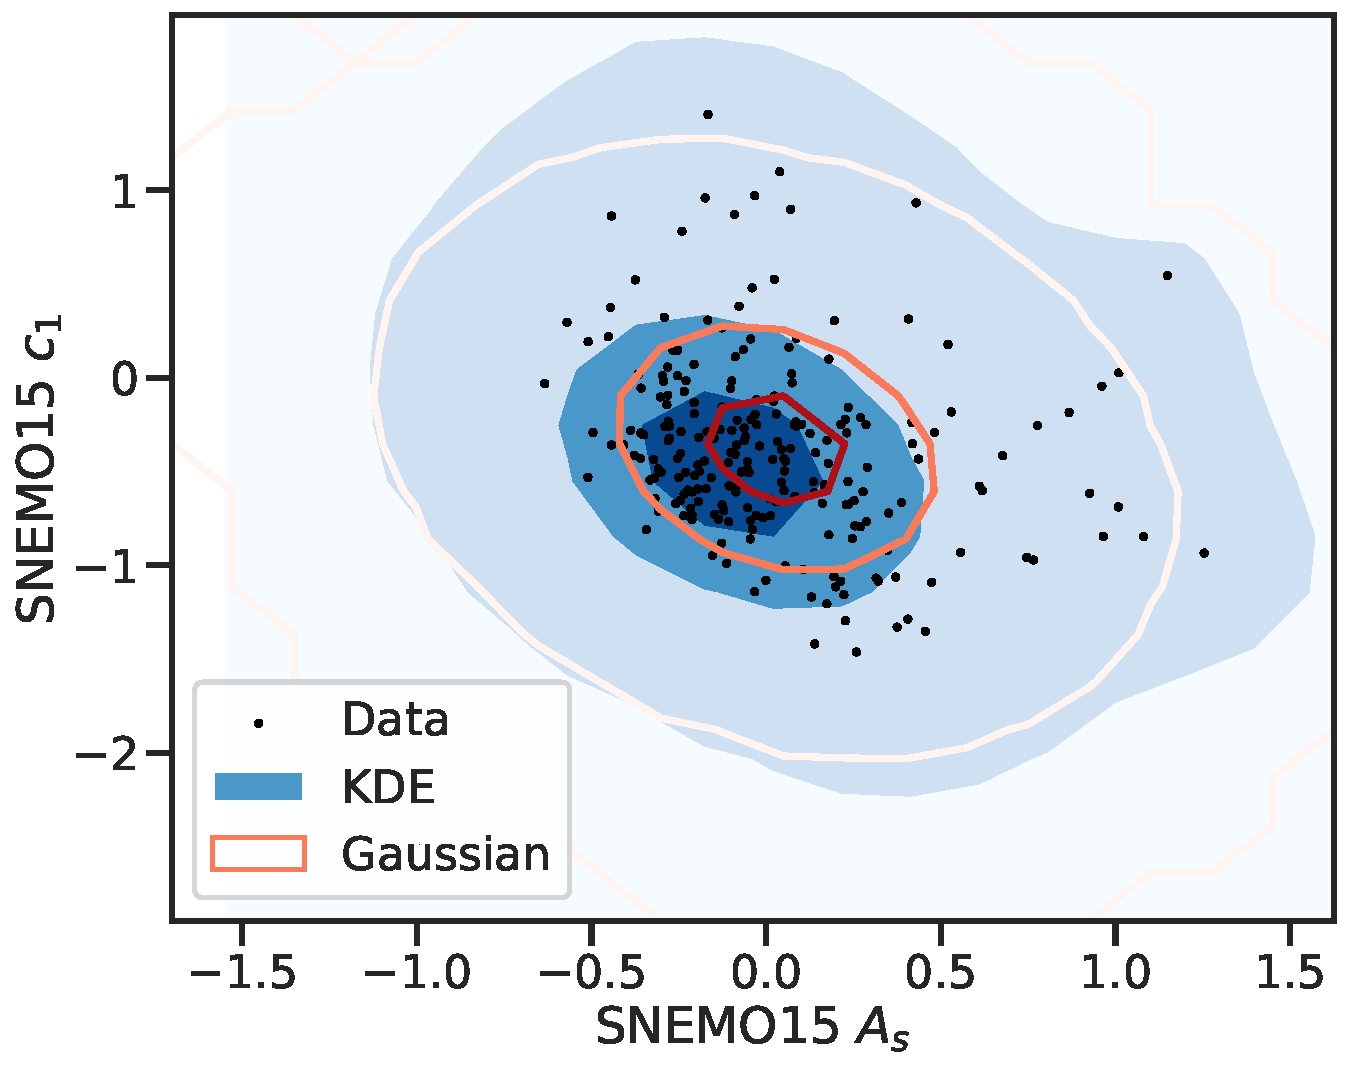
\includegraphics[width=0.6\textwidth]{figures/snemo_kde/snemo15_nongaussian_example.pdf}
%     \caption{Comparison of the KDE estimate (blue filled contours representing the 68th, 95th, and 99th percentiles of samples drawn from the full 16-dimensional estimate) and multivariate Gaussian estimate (similarly spaced red line contours) of the joint probability distribution between SNEMO15 $A_s$ and $c_1$. While the Gaussian estimate shows a closer agreement in the marginal distribution of these parameters, according to the Cram\'{e}r distance (see Fig.~\ref{fig:distances}), the KDE seems to allow a wider variety of values and better captures the skewness of this data because it is not constrained to match the Gaussian form.}
%     \label{fig:snemo15_joint_example}
% \end{figure}

\subsection{Generating Mock Observations}
With the modeled latent space in hand, we can easily obtain new SN~Ia instances to use in further analyses by drawing from the underlying joint probability distribution, calculating the scaling coefficient $x_0$ or $c_0$, and plugging the resulting parameters into Eqn. \ref{eqn:salt_flux_model} or \ref{eqn:snemo_flux_model}. This process gives us a grid of flux values across the model wavelength range (3305-8685~\AA\; for the SNEMO models or 2000-9200~\AA\; for SALT2) and phase range ($-10$ to $+40$ rest-frame days after maximum brightness for the SNEMO models or $-20$ to $+50$ rest-frame days for SALT2).

As explained in Section~\ref{sec:data}, we have modeled the absolute magnitude, rather than the redshift-dependent scaling parameters $x_0$ and $c_0$. To convert the $M_B^* + 19.1$ value to $x_0$ or $c_0$, we first choose a redshift $z$ for the supernova instance based on the needs of our analysis and calculate $m_B$, the peak apparent magnitude of an object at that redshift with $c_0=1$ and all of the remaining parameters set to values determined by the draw from the modeled distribution. We also calculate the desired apparent magnitude, $m_B^*$, by adding the distance modulus $\mu(z)$ from our fiducial cosmology to the apparent magnitude $M_B^*$ drawn from the modeled distribution. The final scale factor is then given by 
$$c_0 = 10^{-0.4(m_B^*-m_B)}.$$

Once we have our grid of flux values $f_{mod}(\lambda, p)$, we can then easily synthesize spectroscopy or photometry of any resolution or signal-to-noise ratio using a tool like \verb|sncosmo|.\footnote{\url{https://sncosmo.readthedocs.io/en/v2.1.x/}} \added{\citep{Barbary:11938}} In Fig.~\ref{fig:example_prism_spec}, we show spectra of an example object at redshift $z=0.775$ with intrinsic flux determined by a draw from the KDE model of the SNEMO15 model parameters, using the spectral resolution of the proposed Roman Space Telescope prism spectrograph and signal-to-noise equivalent to an exposure time of roughly one hour. Fig.~\ref{fig:example_roman_lc} shows the same object but observed through photometry in the band passes proposed for the Roman Wide Field Instrument for a similar exposure time \citep{rubin_evaluating_2020, roman_space_telescope_reference_information_roman_2019}. Code for generating these spectra and light curves is available publicly\footnote{\url{https://github.com/sam-dixon/snemo_generator}}.

\begin{figure}
    \centering
    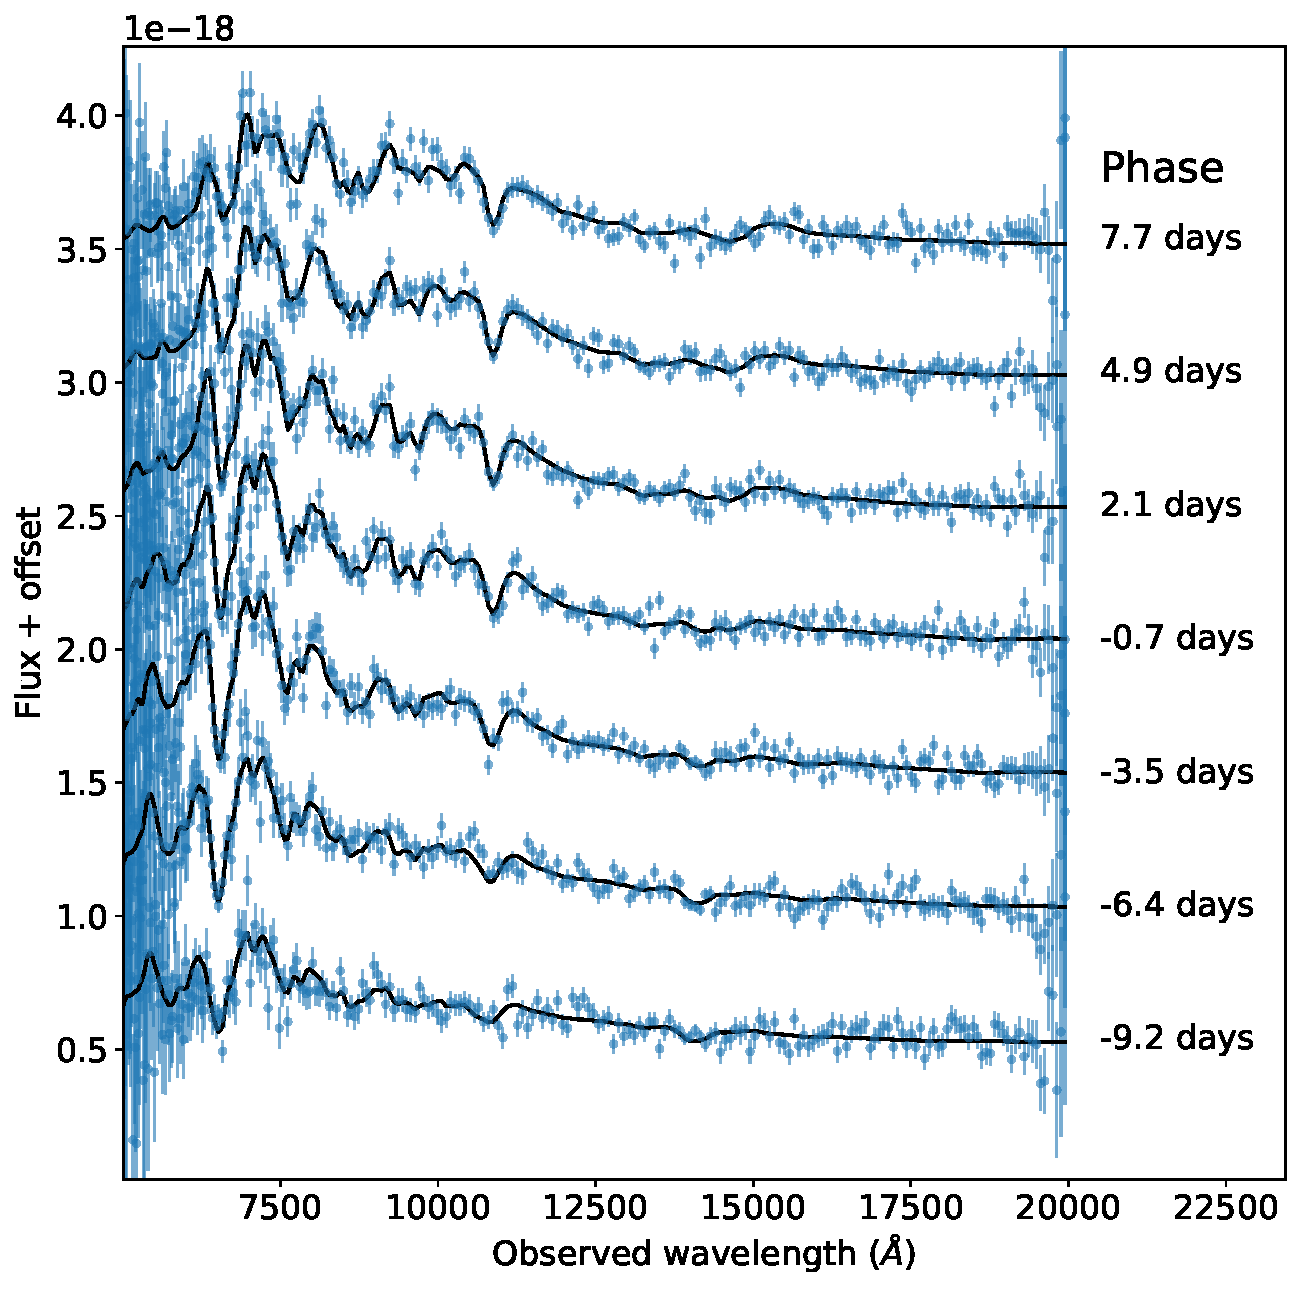
\includegraphics[width=0.9\textwidth]{figures/snemo_kde/example_roman_spec.pdf}
    \caption{A series of synthesized spectral observations at a range of phases for a single object at redshift $z=0.775$ generated from a random draw from the SNEMO15 KDE. The resolution matches the proposed design of the Roman Space Telescope prism spectrograph, and the signal-to-noise ratio representing the level that could be obtained with an hour of exposure time. The black lines represent the underlying spectral energy distribution generated by our model, and the blue points represent the flux values in each prism wavelength bin, along with their associated errors.}
    \label{fig:example_prism_spec}
\end{figure}

\begin{figure}
    \centering
    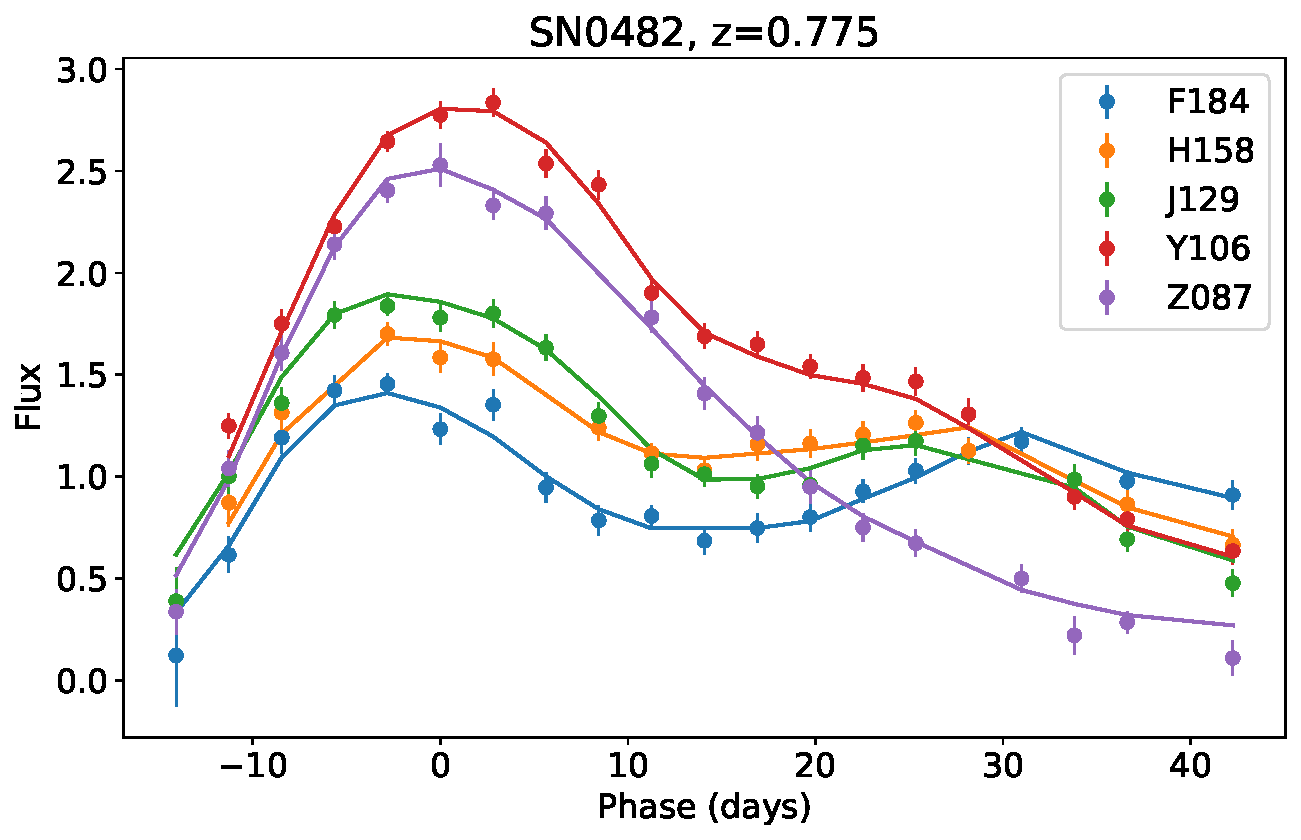
\includegraphics[width=0.9\textwidth]{figures/snemo_kde/example_roman_lc.pdf}
    \caption{Synthetic photometry of the same object shown in Fig.~\ref{fig:example_prism_spec}, but observed photometrically in the Roman Wide Field Instrument bandpasses. Again, the lines represent the underlying flux of the generated supernova. The points represent an example of the noisy observed flux, and its associated errors.}
    \label{fig:example_roman_lc}
\end{figure}

\section{Evaluating Spectral Diversity}
\label{sec:spec_diversity}
As another means of quantifying the usefulness of this tool, as well as a concrete example of the kind of analysis that is uniquely enabled by both a non-parametric model of spectral model parameters and the use of spectral models with more degrees of freedom (i.e. SNEMO7 and SNEMO15), we compare the distributions of several spectral features measured from the training spectra to those obtained with data simulated by the techniques introduced in this work. The development of the SNEMO models was largely motivated by the recognition that spectral models like SALT2 do not capture the full range of spectral variation that is seen in Type Ia supernovae \citep{saunders_snemo_2018}. This study aims to quantify how well higher-dimensional linear models and non-parametric models of the latent parameter space of these linear models can capture the non-linear features that may provide a better understanding of supernova standardization and supernova physics.

We chose to focus on the velocities and pseudo-equivalent widths of the \CaIIHK{} {} doublet, the \SiIIblue{} line, and the \SiIIred{} line at maximum brightness. As discussed in Chapters \ref{chap:intro} and \ref{chap:si_feat_pca}, these spectral indicators are commonly used in studies aiming to improve the standardization of supernova brightnesses beyond light curve shape and color, or to quantitatively subclassify Type Ia supernovae in order to gain a better understanding of their physics. The ejecta velocities of SNe~Ia, measured by the line velocities of \SiIIred{} and \CaIIHK{} {}, have been shown to correlate with their intrinsic colors \citep{foley_measuring_2011, foley_velocity_2011, foley_relation_2012, mandel_type_2014}. The width of the \SiIIred{} line shows a similar correlation \citep{foley_velocity_2011}. All of these relationships can lead to potential redshift-dependent distance bias if left uncorrected. An example subclassification scheme using these parameters is the Branch classification scheme \citep{branch_comparative_2006}, which arranges SNe~Ia by the widths of their \SiIIblue{} and \SiIIred{} lines, showing that there is a wide range in spectral feature behavior within the Ia class. 

For the observed data, we measured these features using a method similar to \cite{blondin_using_2006}, in which we first smooth the spectrum, then define a pseudo-continuum from the local maxima near the features in question. Using the smoothed, pseudo-continuum-removed flux, we use the relativistic Doppler formula to calculate the eject velocities, and integrate the flux to find the pseudo-equivalent width. When making measurements of the spectral features from the generated spectra, we proceed similarly, but skip the smoothing step, as the spectrum is already assumed to be noiseless. Full details of this process are presented in Appendix \ref{app:spec_feat}. 

The spectral indicators were measured from the spectrum of each supernova in our data set that was closest to the SALT2-predicted time of B-band maximum brightness, $t_0$. To minimize the impact of phase evolution of the features, we remove from the analysis all objects that do not have a spectrum within $\pm 5$ rest-frame days of $t_0$. This leaves 213 supernovae. Code to perform these measurements is publicly available through the \verb|spectral_lines| package \footnote{\url{https://github.com/sam-dixon/spectral_lines}}.

\subsection{Comparing Features Measured from Data and from Best-fit Spectral Models}
We would like to separate our quantification of how well the spectral flux models themselves are able to capture the full distributions of spectral features from how closely samples generated from the KDE models of the spectral model parameters mimic the true distribution. To answer the first question, we make measurements of the spectral features from noiseless, at-max spectra synthesized directly from the best-fit spectral model parameters for each supernova and each spectral model. We will refer to these measurements as the model measurements.

Fig.~\ref{fig:model_vSi_recovery} shows histograms of the residuals between these model-measured velocity of \SiIIred{} ($v_{6355}$) and the data-measured velocity for each object in our data set. We can see that as the number of model components increases, the scatter on these residuals decreases, indicating that the increased flexibility of these higher-dimensional spectral models allows them to capture these spectral features. For SNEMO15, the average difference between the model and data measurements of the velocity of this line is comparable in size to the typical measurement error of this feature.

\begin{figure}
    \centering
    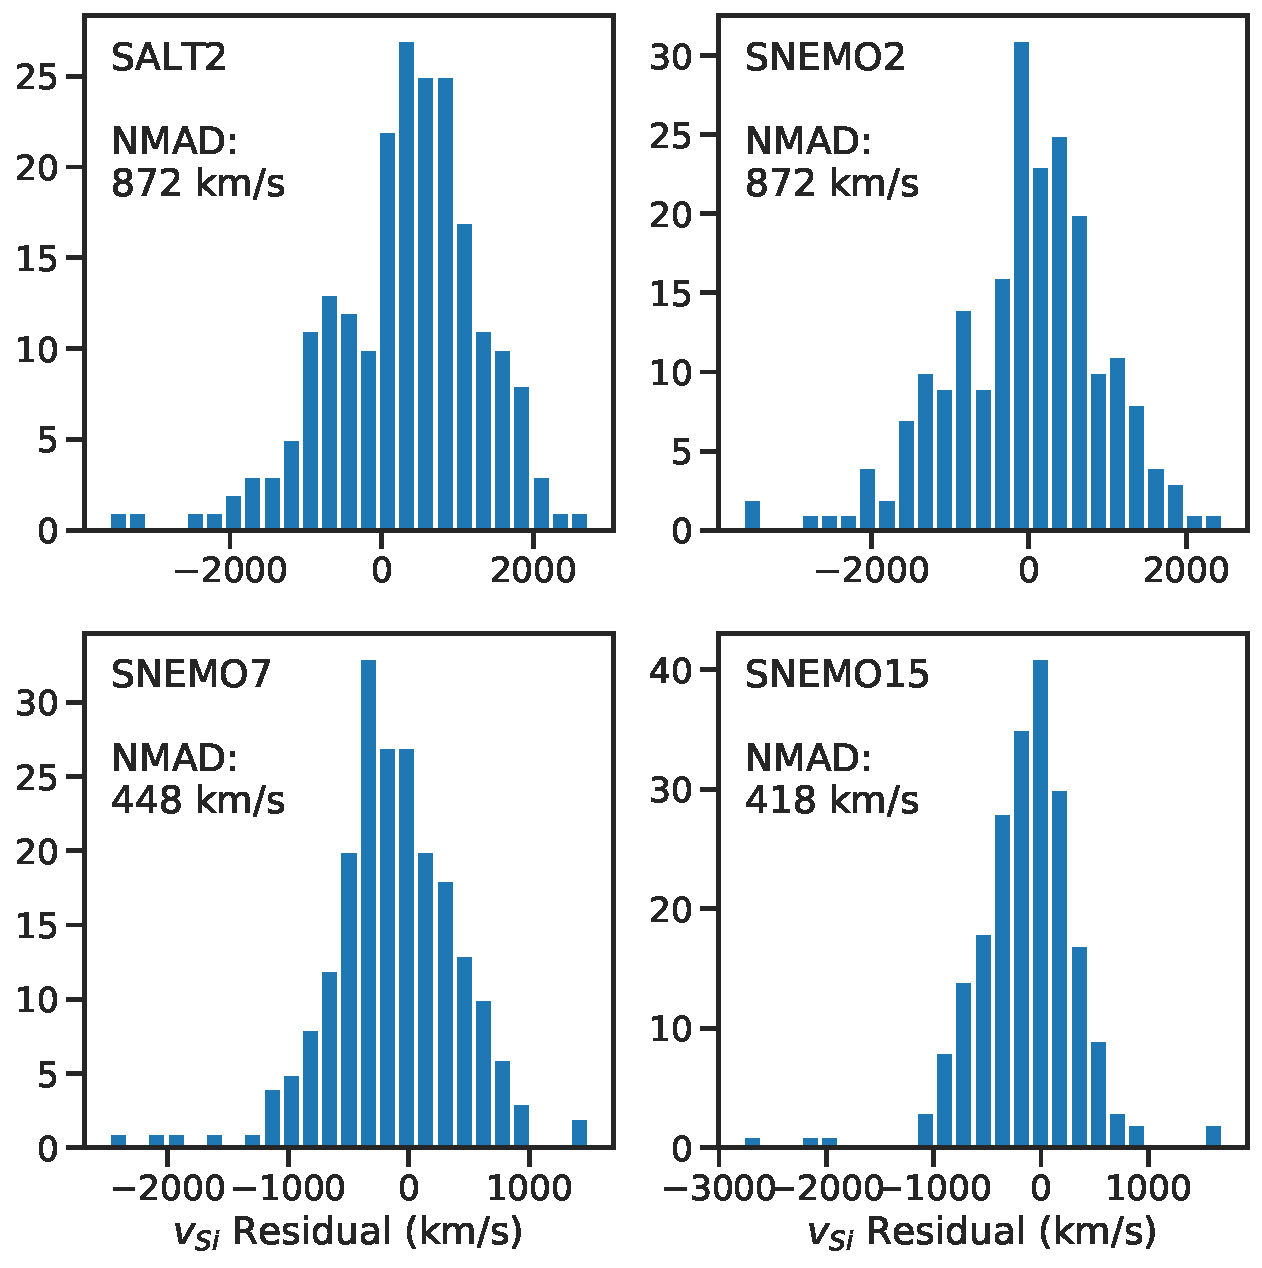
\includegraphics[width=0.9\textwidth]{figures/snemo_kde/model_vSi_recovery.pdf}
    \caption{Histograms of the residuals between the velocity of the \SiIIred{} line as measured from the data and as measured from the spectrum generated with the best-fit spectral model parameters. Lower dimensional models (SALT2 and SNEMO2) }
    \label{fig:model_vSi_recovery}
\end{figure}

This general trend is seen across all the spectral indicators studied, with the exception of the width of the \SiIIblue{} line; we can see this in Fig.~\ref{fig:model_spec_feat_recovery}, where we compare the normalized median absolute deviation (NMAD)\footnote{$\text{NMAD}(\bm{x})=1.4826\;\text{median}(|\bm{x}-\text{median}(\bm{x})|)$} of the residuals between model and data spectra for each spectral indicator across spectral models. It is not immediately obvious why the width of the \SiIIblue{} line is captured nearly as well by SALT2 and SNEMO2 as it is by SNEMO15, but not captured by SNEMO7. It may be due to the fact that it is a relatively small feature, and therefore both more difficult to measure precisely on the data spectrum and poorly sampled in the SNEMO spectral eigenvectors. Regardless, we find that SNEMO15 is the best at capturing all of the spectral indicators that we studied.

\begin{figure}
    \centering
    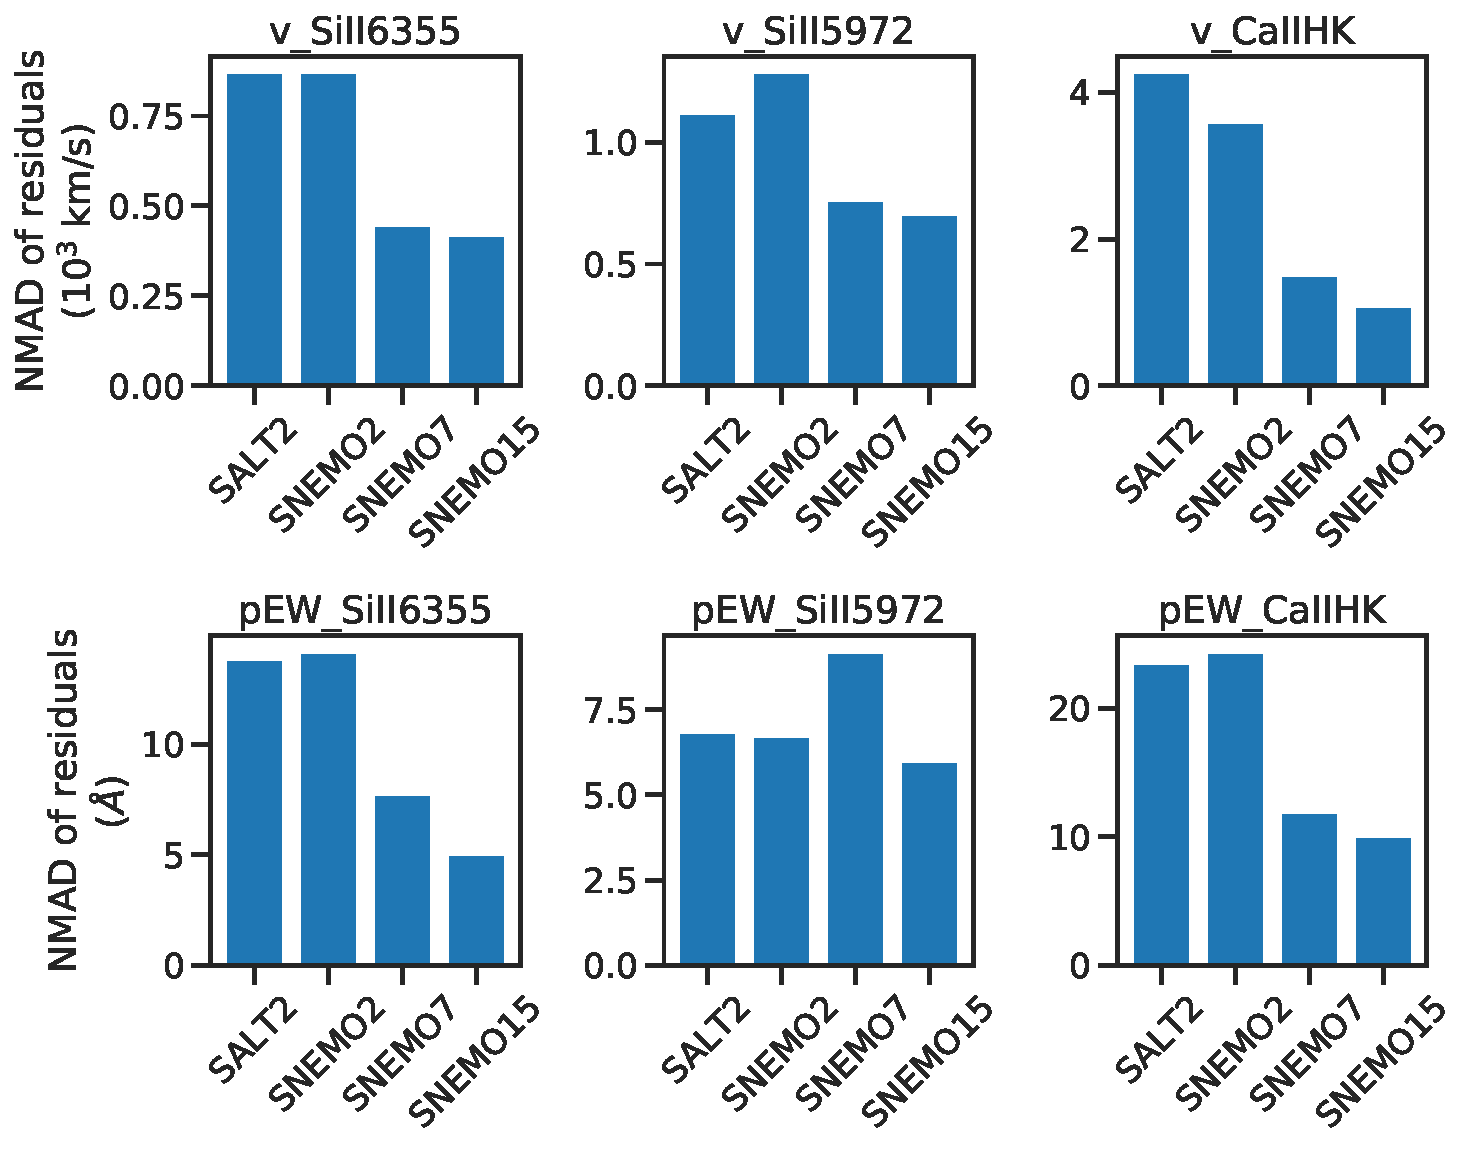
\includegraphics[width=0.9\textwidth]{figures/snemo_kde/model_spec_feat_recovery.pdf}
    \caption{Normalized median absolute deviation of residuals between spectral features measured from data spectra and from spectra generated from the best-fit spectral model. In general, spectral models with more parameters more closely capture the spectral feature measurements.}
    \label{fig:model_spec_feat_recovery}
\end{figure}

\subsection{Comparing Spectral Feature Distributions}
We can also compare the distributions of the spectral indicators measured from spectra generated by the KDE to those measured from spectra in our data set. To do so, we generate 1000 noiseless, at-max spectra from the KDE model of the spectral feature parameters and from a multivariate Gaussian model fit to the same parameters using a standard maximum-likelihood analysis, and measure the same six spectral indicators (velocity and equivalent width of \SiIIred, \SiIIblue, and \CaIIHK{}) for each of these spectra.

The empirical cumulative distributions of the data and the KDE distributions for each of the spectral models are shown in Fig.~\ref{fig:ecdf_kde}. A similar plot, but using the multivariate Gaussian model of the spectral model parameter space, is found in Fig.~\ref{fig:ecdf_gauss}. These figures look quite similar, though we can pick out some differences (like the difference in the lower velocity portion of SNEMO15 distribution of $v_\text{\SiIIblue}$, or the differing relative fractions in each mode of the bimodal $v_\text{\CaIIHK{}}$ distributions for SNEMO15).

\begin{figure}
    \centering
    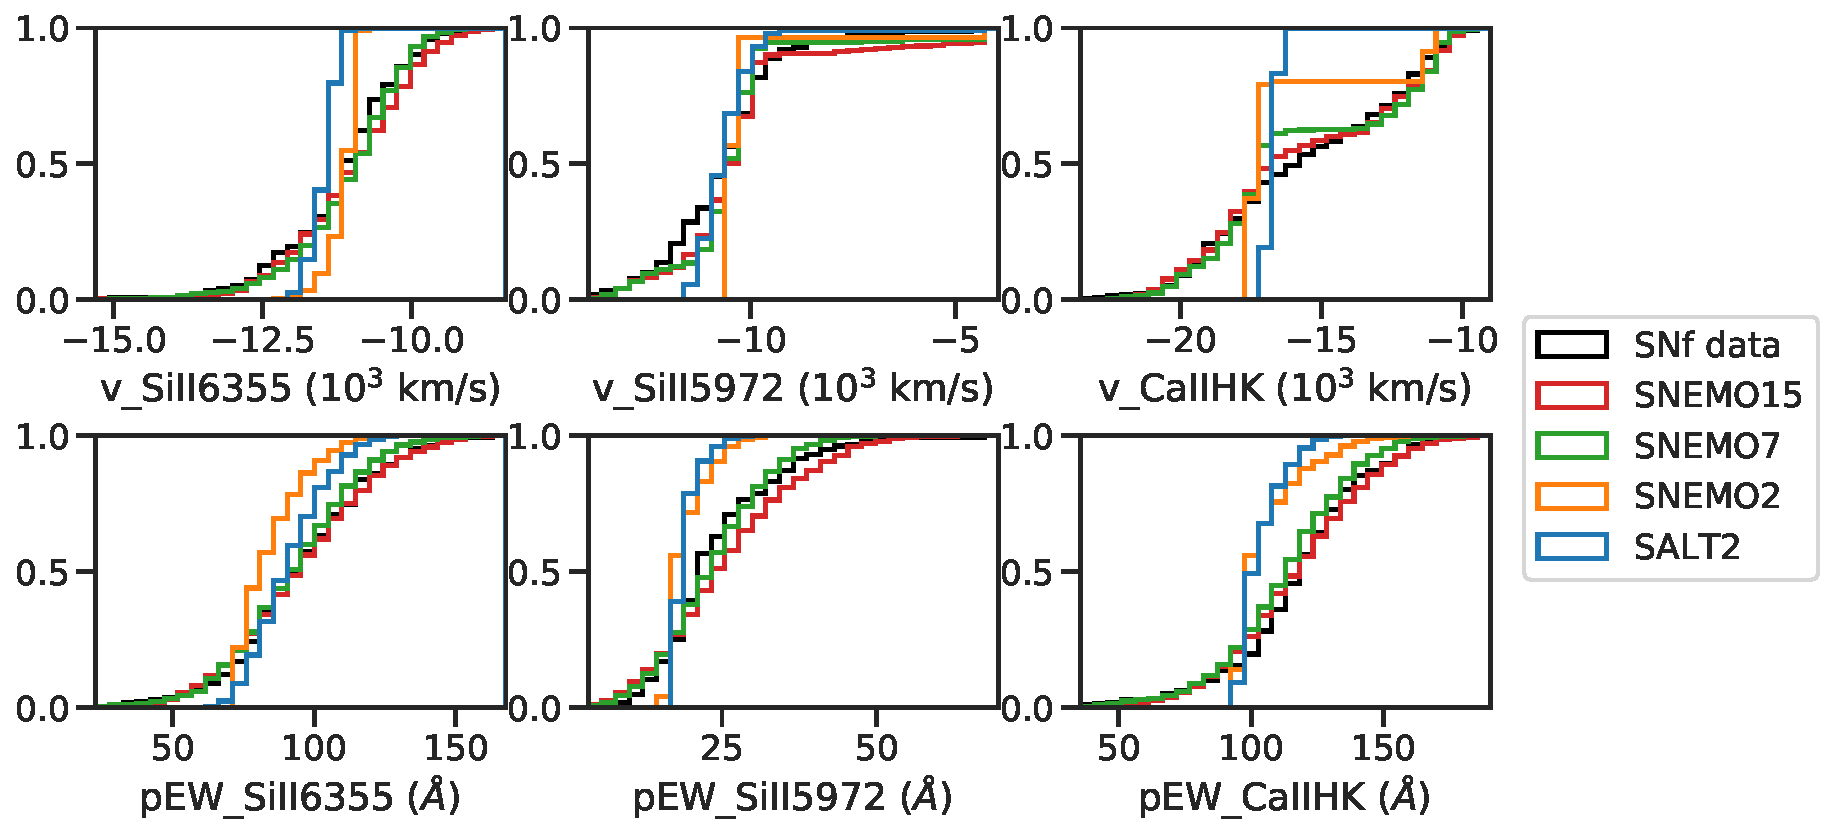
\includegraphics[width=0.9\textwidth]{figures/snemo_kde/ecdf_kde.pdf}
    \caption{Empirical cumulative distribution functions of each spectral indicator for the data set and samples from the kernel density estimate of the spectral model parameter spaces.}
    \label{fig:ecdf_kde}
\end{figure}

\begin{figure}
    \centering
    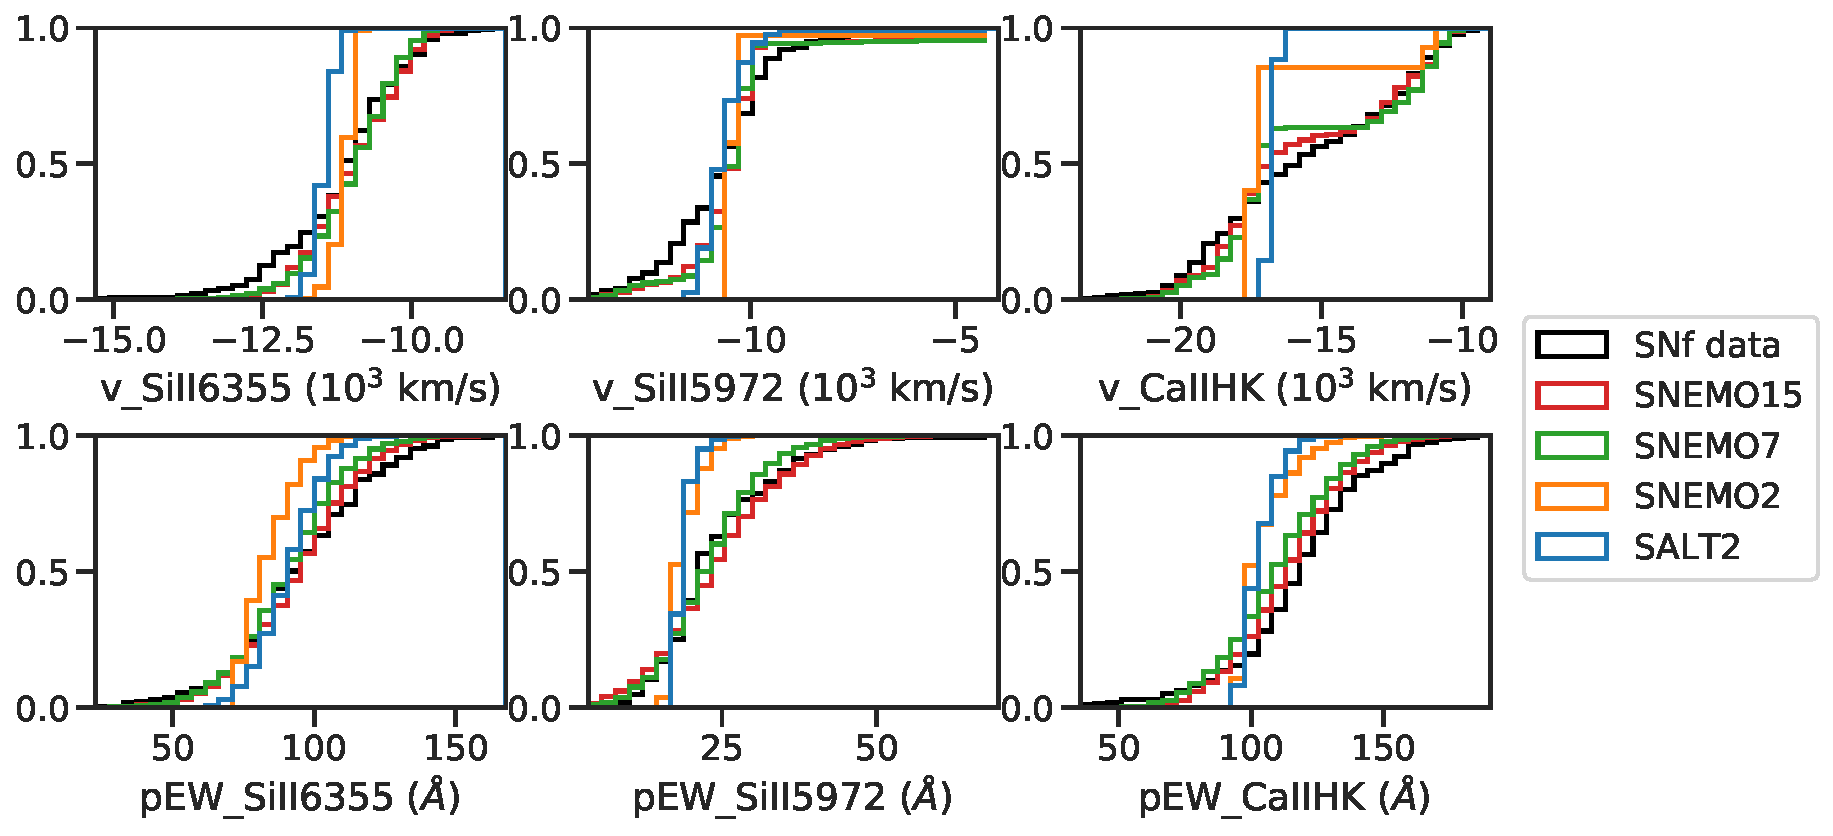
\includegraphics[width=0.9\textwidth]{figures/snemo_kde/ecdf_gauss.pdf}
    \caption{Same as Fig.~\ref{fig:ecdf_kde}, but for samples from the multivariate Gaussian estimation of each of the spectral model parameter spaces.}
    \label{fig:ecdf_gauss}
\end{figure}

% In order to quantify the advantage of using the kernel density estimate over a simpler model (e.g. a multivariate Gaussian) of the joint probability distributions of the spectral model parameters, we use the two-sample Cram\'{e}r distance \citep{cramer_composition_1928} to measure the difference between the cumulative distribution function of the data and the estimated distributions from empirical cumulative distribution functions of the samples.
% The Cram\'{e}r distance $\omega$ between a probability distribution with the empirical cumulative distribution function $F(x)$ and a second probability distribution with the empirical cumulative distribution function $G(x)$ is defined by
% \begin{equation}
%     \omega^2 = \displaystyle \int_\infty^\infty [F(x)-G(x)]^2 dx
% \end{equation}
% Smaller values indicate closer agreement between the two distributions.

% This distance metric has the advantage over other more well-known test statistics (like the Kolmogorov-Smirnov statistic) of being sensitive to differences in the shape of distributions beyond just shifts in the mean or standard deviation, particularly in the tails of the distribution. This is ideal for our task because we want our parameter space estimates to match the true distribution across all portions of parameter space.

We can quantify these differences by calculating the two-sample Cram\'{e}r distances between the distributions of the data and the distributions of the samples for each feature. The Cram\'{e}r distance $\omega$ between a probability distribution with the empirical cumulative distribution function $F(x)$ and a second probability distribution with the empirical cumulative distribution function $G(x)$ is defined by
\begin{equation}
    \omega^2 = \displaystyle \int_\infty^\infty [F(x)-G(x)]^2 dx
\end{equation}
Smaller values indicate closer agreement between the two distributions. This distance metric has the advantage over other more well-known test statistics (like the Kolmogorov-Smirnov statistic) of being sensitive to differences in the shape of distributions beyond just shifts in the global mean or standard deviation, particularly in the tails of the distribution. This is ideal for our task because we want our parameter space estimates to match the true distribution across all portions of parameter space. We can also get obtain an estimate of the error on these distances via bootstrap resampling. 

The calculated Cram\'{e}r distances between the KDE and Gaussian estimates are shown, along with the similarly calculated model-to-data distances, in Fig.~\ref{fig:cramer_spec_feat}. We see a pattern similar to Fig.~\ref{fig:model_spec_feat_recovery} in the spectral feature distribution similarity across models -- in every case, spectral models with more parameters have distributions of the spectral indicators that more closely resemble the data. Additionally, for each of the spectral models, the kernel density estimate of the model parameter distributions creates spectral feature distributions that are as or more similar to the true data distribution than the Gaussian estimates and the best-fit parameter spectra. Overall, this shows that using more flexible spectral models along with more flexible parameter space models allows for a generative model that can accurately reproduce the full range of spectral behavior for simulations.

\begin{figure}
    \centering
    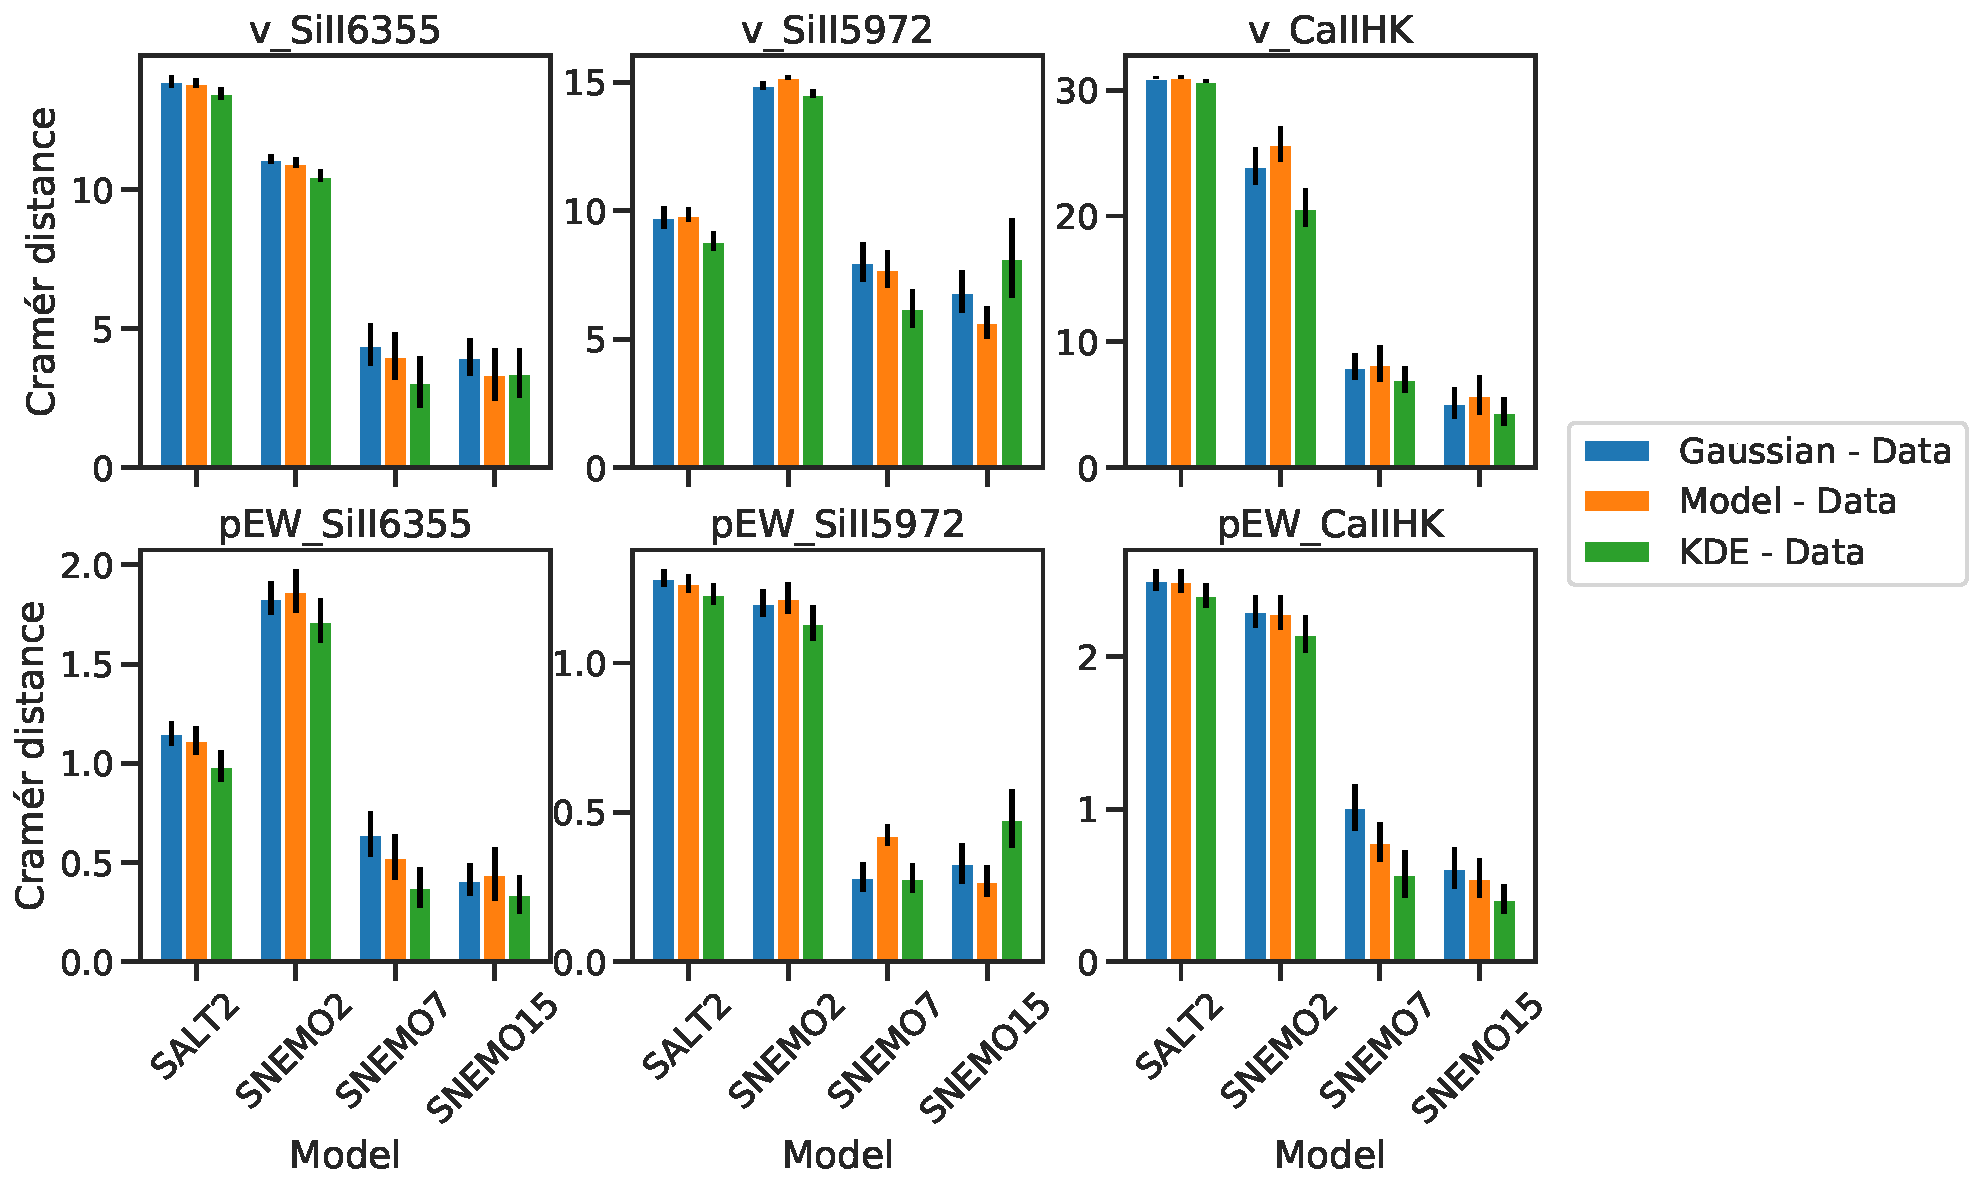
\includegraphics[width=0.9\textwidth]{figures/snemo_kde/cramer_distances_spec_feats.pdf}
    \caption{Cram\'{e}r distances between spectral indicator distributions for the SNfactory data and samples from the Gaussian estimates of the SALT2 and SNEMO parameter distributions, the modeled at-max spectra for the training data, and the KDE estimates of the spectral model parameter distributions.}
    \label{fig:cramer_spec_feat}
\end{figure}

\section{Conclusions}
\label{sec:conclusions}
We have presented flexible estimates of the joint probability distributions of model parameters for the SALT2 and the SNEMO models of \cite{saunders_snemo_2018}. These estimates can be used to generate synthetic spectra and photometry in simulations that exhibit more spectral diversity than current state-of-the-art simulation techniques. This increased variety makes possible a number of different analyses, from examining the robustness of the twinning technique presented in \cite{fakhouri_improving_2015}, to evaluating spectral feature measurement techniques under different observing conditions. There are a number of spectral properties of Type Ia supernovae beyond the two-parameter light curve shape and color parameters that have been shown to ultimately effect our cosmological parameter measurements. This work presents a simulation tool that properly incorporates these variations, allowing us to properly understand their impacts for future cosmological surveys.
